\subsection{Vincoli di cardinalità}

\begin{itemize}
    \item \textbf{Significato}:  
    Data una relazione $R$, i \textbf{vincoli di cardinalità} vengono specificati per ogni entità $E_i$ coinvolta nella relazione $R$ e indicano:
    \begin{itemize}
        \item il \textbf{numero minimo} di istanze di $R$ a cui un’istanza di $E_i$ \textit{deve} partecipare;
        \item il \textbf{numero massimo} di istanze di $R$ a cui un’istanza di $E_i$ \textit{può} partecipare.
    \end{itemize}

    \item \textbf{Sintassi grafica}:  
    I vincoli di cardinalità si specificano sulle linee che collegano ogni entità alla relazione.  
    Per ogni entità $E_i$ si indica una coppia di valori \texttt{(min, max)} accanto al collegamento.
\end{itemize}

\begin{figure}[!h]
    \centering
    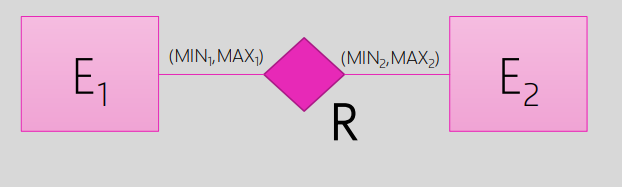
\includegraphics[width=0.5\linewidth]{image10.png}
    \caption{Esempio di vincoli di cardinalità}
    \label{fig:vincoli_cardinalita}
\end{figure}
\subsubsection{Valori possibili per Min}
\begin{itemize}
    \item 0 : indica che la partecipazione alla relazione $R$
delle istanze di $E_i$ è OPZIONALE
    \item 1 : indica che la partecipazione alla relazione $R$ delle istanze di $E_i$ è OBBLIGATORIA
    \item num $>$ 1 : indica che per ogni istanze di $E_i$ devono
essere presenti almeno $<num>$ occorrenze della
relazione $R$ che la coinvolgono

\end{itemize}
\subsubsection{Valori possibili per Max}
\begin{itemize}
    \item 1 :indica che un’istanza di $E_i$ può al massimo
partecipare a una sola occorrenza della relazione
$R$ (se $R$ è binaria questo indica che $R$ è una
\textit{FUNZIONE})
    \item N : indica che un’istanza di $E_i$ può partecipare a più occorrenze della relazione $R$ senza limite massimo
    \item $num > 1$ : indica che per ogni istanza di $E_i$ possono essere presenti al più $<num>$ occorrenze della relazione $R$ che la coinvolgono
\end{itemize}
\subsubsection{Esempio:}
Supponiamo di aver inserito nello schema le entità
$PERSONA$ e $COMUNE$, e ipotizziamo che nei
requisiti sia indicata la necessità di gestire la
$RESIDENZA$ delle persone nei comuni italiani.
Rappresento con il costrutto relazione il concetto
di $RESIDENZA$.
\begin{figure}[!h]
    \centering
    
\includegraphics[width=0.75\linewidth]{image11.png}
    \caption{Esempio}
    \label{fig:placeholder}
\end{figure}

\begin{tcolorbox}[colback=yellow!15!white, colframe=orange!80!black, title=\textbf{Kristian semplifica in questo modo}]
Le \textbf{cardinalità} si possono leggere come un intervallo “\textbf{da–a}”:  
\begin{itemize}
    \item Il primo valore (\textbf{min}) indica \textbf{da quante volte almeno} un’entità partecipa alla relazione.  
    \item Il secondo valore (\textbf{max}) indica \textbf{quante volte al massimo} può partecipare.
\end{itemize}

\begin{center}
\begin{tabular}{|c|c|c|}
\hline
\textbf{Cardinalità} & \textbf{Significato} & \textbf{Lettura “da–a”} \\
\hline
(0,1) & Facoltativa e singola & da 0 a 1 volta \\
(1,1) & Obbligatoria e singola & da 1 a 1 volta \\
(0,N) & Facoltativa e multipla & da 0 a N volte \\
(1,N) & Obbligatoria e multipla & da 1 a N volte \\
\hline
\end{tabular}
\end{center}
\end{tcolorbox}

